\begin{frame}{Nonrandom connectivity from anisotropy}
  % 
  \begin{columns}
    % 
    \begin{column}{.45\textwidth}
      \minipage[c][0.75\textheight][s]{\columnwidth}
      
      \begin{figure}
        \centering
        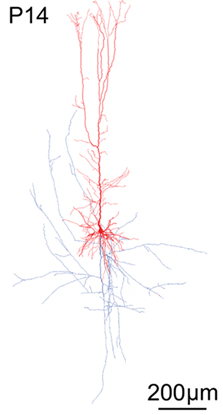
\includegraphics[width=\textwidth]{%
          figures/Romand2011_P14_1.png} %
      \end{figure}
      
      
      \endminipage      
    \end{column}
    % 
    \begin{column}{.55\textwidth}


      \vspace{-0.2cm}
      
      \begin{figure}
        \centering
        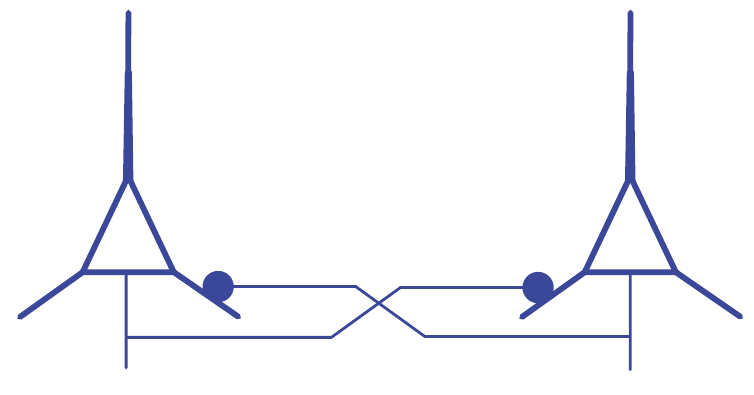
\includegraphics[width=0.525\textwidth]{%
          figures/two_neuron.png} %
      \end{figure}

      \vfill
      

      \begin{figure}
        \centering
        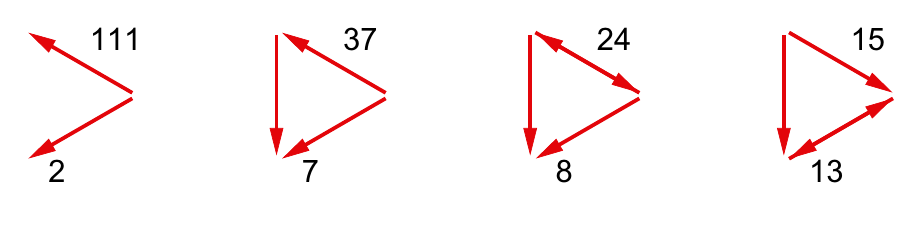
\includegraphics[width=\textwidth]{%
        figures/Perin2011_FigS2_custom.png} %
      \end{figure}

      \vfill
      

      \begin{figure}
        \centering
        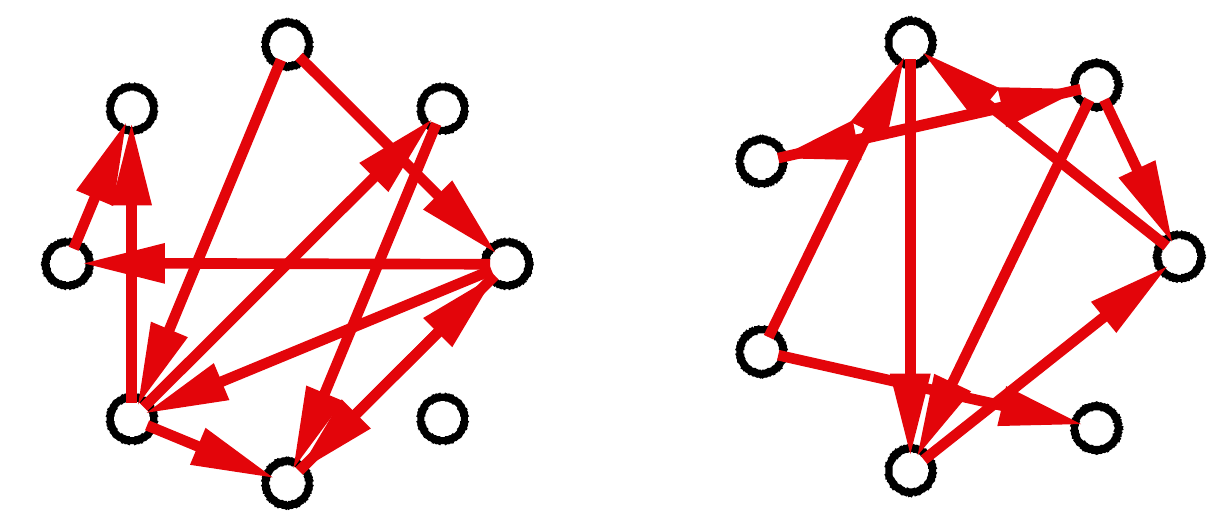
\includegraphics[width=0.7\textwidth]{%
          figures/clust_all.png} %
      \end{figure}
      
      \vfill

      
    \end{column}
  \end{columns}

  % \source{\cite{Perin2011, Song2005, Markram1997, Miner2016, Gal2017,
  %     Vegue2017}}

  \pnote{
    
    These nonrandom structures are well established and have been reported both, 
    
  }
  
\end{frame}


